\section{Introducción Teórica}

El objetivo de este trabajo es encontrar la inversa de la raíz cuadrada de un
número, de forma eficiente. Para esto analizamos dos funciones diferentes cuyos
ceros nos ayudarán a encontrar la inversa de la raíz deseada. Estas dos
funciones son:

\begin{equation}\label{f_x}
    f(x) = x^2 - \alpha
\end{equation}

\begin{equation}\label{e_x}
    e(x) = \frac{1}{x^2} - \alpha
\end{equation}

En este trabajo sólo estudiaremos el dominio de los reales $\Re$. Debido
a esto, el dominio de estas funciones en el cual estamos interesados es $\alpha
> 0$ ya que en $\Re$ la raíz cuadrada solo se puede aplicar a números
positivos y no existe la división por $0$.

Para encontrar los puntos en que las funciones se anulan utilizaremos los
métodos iterativos de Newton y de la Secante.

\subsection{Análisis de $f(x)$}\label{sec:analisis_f_x}

\begin{figure}[h]
  \begin{center}
    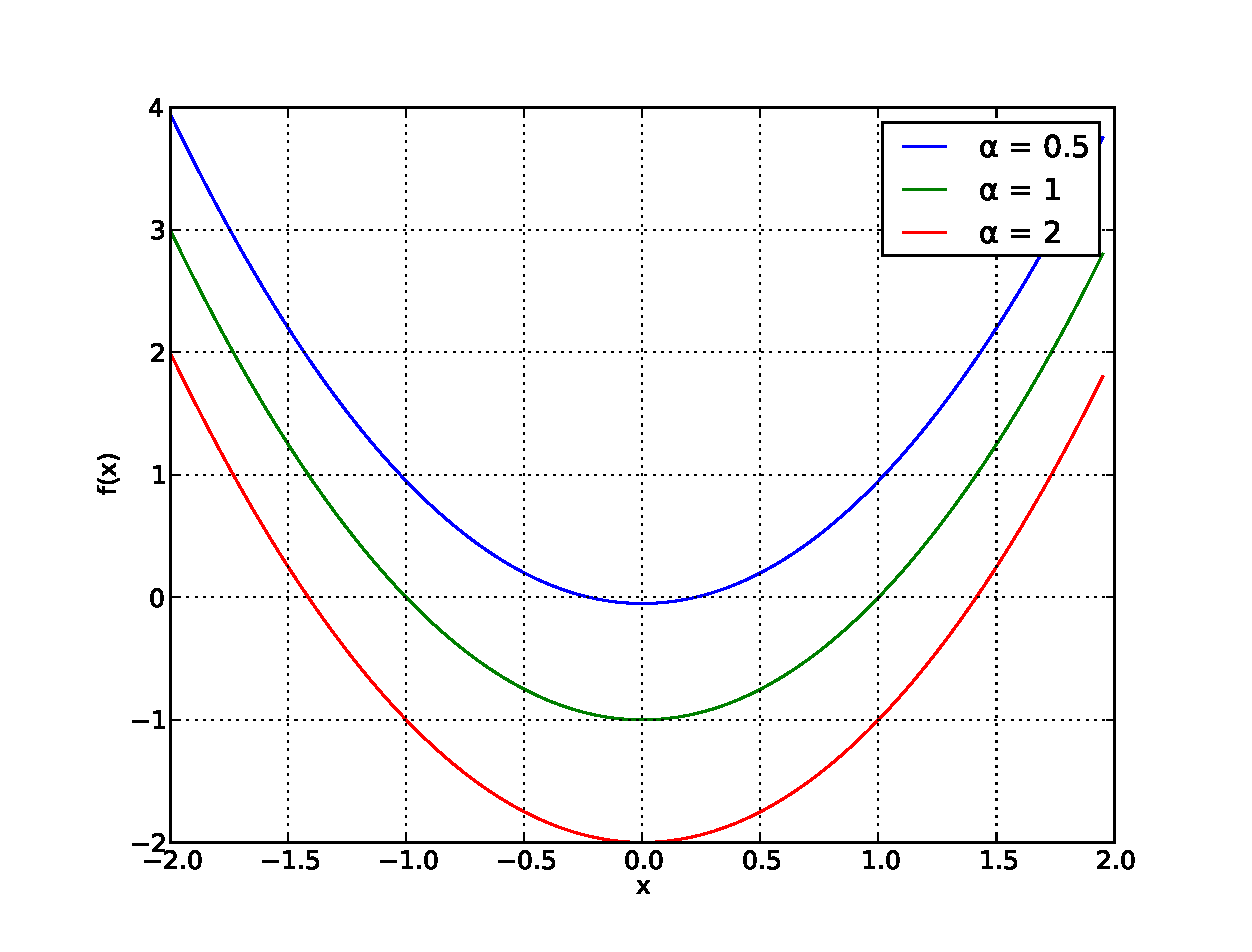
\includegraphics[scale=0.5]{graficos/new/f_x.eps}
    \caption{\label{fig:f_x} Gráfico de $f(x)$ variando $\alpha$.}
  \end{center}
\end{figure}

Llamemos $\displaystyle \beta = \frac{ 1 }{ \alpha }$. $\beta$ es el número al
cual le queremos encontrar la inversa de la raíz cudarada.

Por otro lado la expresión de $f(x)$ la podemos reescribir de esta manera:

\[
    f(x) = x^2 - \alpha = (x + \sqrt{\alpha})(x - \sqrt{\alpha})
\]

Podemos ver que esta es una función cuadrática y que tiene dos raíces diferentes.

Estas raíces existen pues $\alpha > 0$ y como podemos ver las raíces son
iguales en módulo y nos sirven para hallar $\beta$. Si la raíz encontrada es
negativa simplemente cambiando el signo obtendremos la raíz en la cual estamos
interesados. Por lo tanto:

\[
    x = \sqrt{\alpha} \implies \beta = \frac{ 1 }{ x }
\]

$f(x)$ es convexa ya que su derivada segunda es $f''(x) = 2$.

\subsection{Análisis de $e(x)$}\label{sec:analisis_e_x}

\begin{figure}[h]
  \begin{center}
    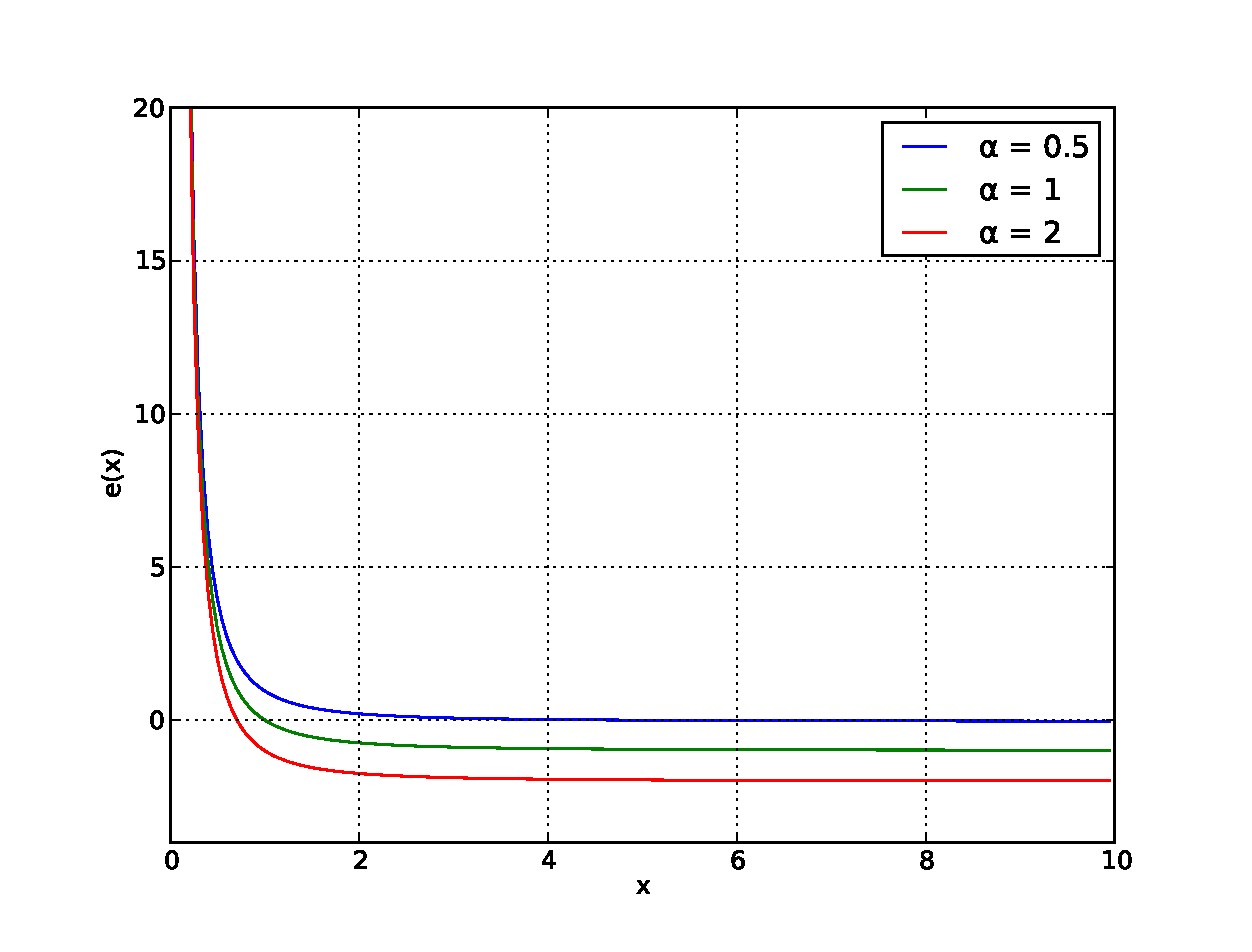
\includegraphics[scale=0.5]{graficos/new/e_x.eps}
    \caption{\label{fig:e_x} Gráfico de $e(x)$ variando $\alpha$.}
  \end{center}
\end{figure}

Reescribamos $e(x)$ de la siguiente forma:

\[
    e(x) = 0 \implies
    \frac{ 1 }{ x^2 } - \alpha = 0 \implies
    \frac{ 1 }{ x^2 } = \alpha \implies
    x^2 = \frac{ 1 }{ \alpha } \implies
    x = \frac{ 1 }{ \sqrt{\alpha} }
\]

Se puede ver que al encontrar las raíces de $e(x)$ encontramos lo deseado, la
inversa de la raíz cuadrada de $\alpha$.

$e(x)$ con $\alpha > 0$ tiene dos raíces diferentes de mismo módulo, por lo que
al igual que en el caso de $f(x)$ nos es indistinto cuál de las dos
encontremos, ya que cambiando el signo obtenemos la otra raíz.

Esta función tiene dos asíntotas. En el eje de las ordenadas podemos encontrar
una en $x = 0$, mientras que en el eje de las abscisas podemos encontrar una
asíntota en $e(x) = - \alpha$ cuando $x \to \pm \infty$.

\subsection{Método de Newton}

El método de Newton es un método iterativo para buscar aproximaciones
sucesivamente mejores de las raíces de una función real $h(x)$.

Para aplicar este método es necesario que exista y conocer la derivada de la
función a analizar en un intervalo real $[a, b]$.

Dado un $x_0$ inicial suficientemente cerca de la raíz deseada, se pueden
obtener sucesivas mejores aproximaciones a partir de:

\begin{equation}\label{newton}
    x_{n + 1} = x_n - \frac{ h(x_n) }{ h'(x_n) }
\end{equation}

La ``idea gráfica'' de este método es empezar un por un punto ($x_0$), luego
obtener la tangente de la función en ese punto y obtener el siguiente punto
(una mejor aproximación) donde la recta tangenta intersecta el eje de las
abscisas.

El órden de convergencia de este método es cuadrático siempre y cuando la
multiplicidad de la raíz buscada sea 1. En el caso de las funciones $f(x)$ y
$e(x)$ esto es así y podemos obtener sus derivadas:

\begin{equation}\label{f1_x}
    f'(x) = 2x
\end{equation}

\begin{equation}\label{e1_x}
    e'(x) = -\frac{2}{x^3}
\end{equation}


\subsubsection{Convergencia para $f(x)$}\label{sec:convergencia}

Veamos que Newton siempre converge para $f(x)$ si $x_0 > \sqrt{\alpha}$.

Utilizaremos una demostración inductiva. El paso iterativo de Newton para
$f(x)$ se puede escribir de la siguiente forma:

\[
    x_{n + 1} = \frac{ 1 }{ 2 } ( x_n + \frac{ \alpha }{ x_n })
\]

{\bf Inducción en k $\in \mathbb{N}$}

Queremos probar que si $x_0 > \sqrt{\alpha}$ entonces $\sqrt{\alpha} < x_{k + 1}
< x_k$, es decir, $x_{k + 1}$ se encuentra más cerca de la raíz que $x_k$.

{\bf Caso base: $P(0)$}

Sea $k = 1$, queremos ver que $x_1 < x_0$. Entonces reemplazando $x_1$ por su definición tenemos:

\begin{align*}
    x_1 < x_0 &\iff \\
    \frac{1}{2}(x_0 + \frac{\alpha}{x_0}) < x_0 &\iff \\
    x_0 + \frac{\alpha}{x_0} < 2x_0 &\iff \\
    \frac{\alpha}{x_0} < x_0 &\iff \\
    \alpha < x_0^2 &\iff \\
    \sqrt{\alpha} < x_0&
\end{align*}

Y esto último es la precondición. Por lo tanto $x_1 < x_0$ $_\square$

Veamos también que $x_1 > \sqrt{\alpha}$

\begin{align*}
    x_1 > \sqrt{\alpha} &\iff \\
    \frac{1}{2}(x_0 + \frac{\alpha}{x_0}) > \sqrt{\alpha} &\iff \\
    x_0 + \frac{\alpha}{x_0} > 2\sqrt{\alpha} &\iff \\
    x_0 - 2\sqrt{\alpha} > -\frac{\alpha}{x_0} &\iff \\
    x_0^2 - 2\sqrt{\alpha}x_0 + \alpha > 0 &\iff \\
    {(x_0 - \sqrt{\alpha})}^2 > 0
\end{align*}

Luego esto último vale pues $x_0 > \sqrt{\alpha}$. Por lo tanto, por esto y por lo demostrado antes vale que:

\[
    \sqrt{\alpha} < x_1 < x_0
\]

{\bf Caso n + 1: $P(n) \implies P(n + 1)$}

Sea $k = n + 1$. Veamos que $x_{n + 1} < x_n$.

Podemos escribir $x_{n + 1}$ como:

\begin{align*}
    x_{n + 1} = \frac{ 1 }{ 2 }(x_n + \frac{ \alpha }{ x_n }) = \frac{ x_n^2 + \alpha }{ 2x_n }
\end{align*}

Por {\bf HI} vale que $\sqrt{\alpha} < x_n \iff \alpha < x_n^2 $ Entonces:

\[
    \frac{ x_n^2 + \alpha } {2x_n } < \frac{ x_n^2 + x_n^2 }{ 2x_n } = x_n
\]

Por lo tanto $x_{n + 1} < x_n$

Ahora veamos que $\sqrt{\alpha} < x_{n + 1}$:

\[
    \sqrt{\alpha} < x_{n + 1} \iff \sqrt{\alpha} < \frac{1}{2}(x_n + \frac{\alpha}{x_n}) \iff
\]

\[
     \sqrt{\alpha} < \frac{x_n^2 + \alpha}{2x_n} \iff 2x_n\sqrt{\alpha} < x_n^2 + \alpha \iff
\]

\[
     0 < x_n^2 - 2x_n\sqrt{\alpha} + \alpha \iff 0 < {(x_n - \sqrt{\alpha})}^2
\]

Y esto último vale ya que por {\bf HI} $\sqrt{\alpha} < x_n$. Por lo tanto demostramos que:

\[
    \sqrt{\alpha} < x_n < x_{n - 1} \square
\]

\subsection{Método de la Secante}

El método de la Secante es un método iterativo para buscar aproximaciones
sucecivamente mejores de las raíces de una función real $h(x)$. Se puede ver
como una derivación del método de Newton donde no es necesario conocer la
derivada de la función, sino que esta se aproxima utilizando la aproximación de
diferencias finitas. Su paso iterativo es:

\begin{equation}\label{secante}
    x_{n + 1} = x_n - h(x_n) \frac{ x_n - x_{n - 1} }{ h(x_n) - h(x_{n - 1}) }
\end{equation}

La ``idea gráfica'' de este método es similar a la del método de Newton, pero en
este caso, ``aproximar'' la tangente en un punto por la recta que interseca a la
función en $x_0$ y $x_1$.

Su orden de convergencia es supralineal, específicamente es $\phi \approx
1.618$.

Al tener un peor orden de convergencia que el método de Newton requiere de más
pasos para converger, pero al no necesitar calcular la derivada de la función
en la práctica podría ser más veloz.

\subsection{Hipótesis}

En base a este análsis teórico de las funciones y los métodos llegamos a la
idea de que los resultados se comportarán de la siguiente forma. Primero al
haber calculado la derivada de $f(x)$ y de $e(x)$, y por consiguiente poder
utilizar el método de Newton, creemos que este convergerá en una menor cantidad
de iteraciones que el método de la Secante debido a su mejor convergencia
teórica.

Por otro lado, en teoría el método de la secante realiza menos cuentas al no
tener que calcular la derivada en cada iteración, pero en la práctica dependerá
de la implementación.

Por último creemos que $f(x)$ convergerá más rápido para una gran cantidad de
$\alpha$ que $e(x)$ ya que las pendientes de las tangentes en $f(x)$ son más
suaves que las pendientes de las tangentes en $e(x)$. La primera es una
parábola, mientras que la segunda tiene asíntotas muy marcadas, y una vez el
método se encuentre en una de estas asíntotas le costará mucho ``salir'' de
estas, produciendo una convergencia más lenta al resultado.
